\section{Introduction}



\subsection{Background and Motivation}
The \gls{NFC} is a complex system of facilities and material 
mass flows that combine to provide nuclear energy, usually in the form of electricity 
\cite{yacout_modeling_2005}. 
\gls{NFC} simulators are system analysis tools used to investigate 
issues related to the dynamics of a nuclear fuel cycle in both 
high and low-resolution. 
An example of a high-resolution element is the spent fuel 
isotopic composition from a single fuel bundle, and an example 
of a low-resolution element is the total fuel utilization in 
the system. 
The intention behind the use of \gls{NFC} simulators is to develop 
a better understanding of the dependence between various components 
in the system and the effects of changes on the system. 
Their goal is to assist in evaluating and improving potential 
strategies for nuclear power development in terms of improving waste 
management, economic competitiveness, etc. \cite{yacout_modeling_2005}.   

One of the major functionalities of an \gls{NFC} simulator is its 
ability to transmute nuclear fuel in a reactor based on reactor 
conditions such as burnup, enrichment, etc. 
The transmutation results impact the accuracy of the \gls{UNF} 
composition, and thus the capability of using the \gls{NFC} to 
analyze the impact of an \gls{NFC} on variables such as waste profile.  

Current fuel cycle simulators include 
\Cyclus \cite{huff_fundamental_2016},
DYMOND \cite{yacout_modeling_2005},
VISION \cite{jacobson_verifiable_2010},
ORION \cite{gregg_analysis_2012}, 
COSI \cite{coquelet-pascal_cosi6:_2015}, 
and CLASS \cite{mouginot_class_2012}, 
NFC simulators obtain transmutation results using 
various methods.  
Four types of methods to obtain transmutation 
results exist: recipe-based, library-based, spectral, and dynamic 
coupling methods. 
In recipe-based methods, direct neutronics calculations are not performed 
within the model, they are done externally \cite{yacout_vision_2006}. 
The user inputs resulting fresh and spent fuel compositions for specific 
parameters directly into the \gls{NFC} model \cite{sunny_transition_2015}. 
In the library-based method,  the \gls{NFC} simulator dynamically 
calculates depleted fuel recipes by interpolating reactor data libraries 
generated by reactor physics burnup calculation code such as SERPENT 
\cite{leppanen_serpent_2013}, \gls{ORIGEN} \cite{croff_users_1980}, etc. 
In spectral methods, a reactor model that incorporates spectral 
changes as a function of burnup is used \cite{scopatz_essential_2011}. 
In dynamic coupling methods, a \gls{FCS} is coupled with a reactor 
physics depletion code and a depletion calculation is conducted 
during an \gls{NFC} simulation to obtain time-dependent 
transmutation results. 

Table \ref{tab:nfcs} shows a simple breakdown of the 
transmutation methods available for each \gls{NFC} code. 

\begin{table}[h]
    \centering
    \begin{tabular}{|l|l|}
        \hline
        \textbf{\gls{NFC} code} & \textbf{Transmutation Methods Available} \\
        \hline
        \Cyclus \cite{huff_fundamental_2016}& \shortstack[l]{Recipe-based, library-based, \\ spectral, and dynamic-coupling}\\
        \hline
        ORION \cite{gregg_analysis_2012}& Recipe-based and library-based\\
        \hline
        DYMOND \cite{yacout_modeling_2005}& Recipe-based  \\
        \hline
        VISION \cite{jacobson_verifiable_2010}& Recipe-based  \\
        \hline
        COSI \cite{coquelet-pascal_cosi6:_2015} & Recipe-based, library-based, and dynamic coupling\\
        \hline
        CLASS \cite{mouginot_class_2012} & Library-based\\
        \hline
    \end{tabular}
    \caption{Methods for transmutation in reactor modules
             for each \gls{NFC} simulation code. 
             \label{tab:nfcs}}
\end{table}

\Cyclus has three methods to obtain spent fuel compositions: the \Cycamore 
recipe reactor \cite{huff_extensions_2014}, CyBORG 
\cite{skutnik_cyborg_2016}, and Bright-lite \cite{flanagan_brightlite_2014}.  
The \Cycamore recipe reactor accepts a fresh and spent fuel recipe that is 
defined by the user. 
CyBORG uses \gls{ORIGEN} to dynamically calculate depleted fuel recipes 
by interpolating \gls{ORIGEN} reactor data libraries to problem-specific 
conditions including initial enrichment, burnup, and user-specified 
interpolation parameters \cite{skutnik_cyborg_2016}.
Bright-lite uses an interpolated transmutation matrix approach with 
pre-configured libraries available for multiple commercial reactor types
\cite{flanagan_brightlite_2014}. 
This is a spectral type transmutation method. 
ORION has a recipe-based and library-based method to obtain transmutation results. 
In ORION's library-based method, burnup-dependent cross-section libraries 
for multiple reactor types with multiple initial fuel enrichment are 
generated before ORION analysis \cite{sunny_transition_2015}. 
The libraries are then used to generate spent fuel recipes based on 
reactor conditions such as burnup, enrichment, etc.  
DYMOND has a recipe-based method in which recipes for both the input 
and output fuel compositions are externally calculated. 
Isotopes are tracked in lumped categories: fission products, minor 
actinides, uranium and plutonium \cite{feng_standardized_2016}.  
VISION has a recipe-based method with a limited set of
individually tracked isotopes \cite{yacout_vision_2006}. 

For \gls{NFC} simulators, striking a balance between fidelity 
and computational cost is a key issue. 
The advantage of using high fidelity models (dynamic coupling 
methods) is their inherent flexibility 
to readily accommodate varying fuel compositions 
when modeling complex scenarios \cite{sunny_transition_2015}. 
However, using high fidelity models for century-long simulations 
can result in impractical computational times. 
The advantage of using low fidelity models (recipe-based methods)
is the low computational cost. 
They are acceptable methods for modeling fuel cycles with fixed input 
composition or fuel cycles at equilibrium \cite{sunny_transition_2015}. 
However, for fuel cycles not at equilibrium, they result in less 
accurate results. 

Therefore, to find a middle ground of accurate depletion data while 
maintaining a practical computational cost, this paper introduces 
a trained dense neural network model that is able to predict \gls{PWR} \gls{UNF}
composition based on initial enrichment and burnup. 

\subsection{Previous Work}
In 2015, Leniau et al. \cite{leniau_neural_2015} used neural networks
for modeling \gls{MOX} fuel in the \gls{FCS} CLASS. They successfully
demonstrated an application of neural networks to predict plutonium
fraction in a fresh \gls{MOX} fuel required to reach a specific burnup,
as well as to predict mean cross section for depletion calculations.
This work differs from the work by Leniau et al., since it predicts
\gls{UOX} fuel depletion, and the neural network predicts the depleted
compositions directly, which eliminates the need to solve the Bateman
equations. Also, we further extend the concept pioneered by
Leniau et al. by using the trained neural network
to predict a time-aggregated \gls{UNF} inventory, and comparing
the inventory with a pre-existing database. Lastly, this work
implements the neural network to a reactor model to
simulate dynamic (burnup, enrichment) reactor behavior.


\subsection{\Cyclus}

\Cyclus is an agent-based nuclear fuel cycle simulation framework 
\cite{huff_fundamental_2016}, meaning
that each reactor and fuel cycle facility is modeled as a discrete and independent
player in the simulation.
A \Cyclus agent archetype defines the logic that governs the behavior
of an agent. 
\Cyclus archetypes are implemented in  either \CC  or Python.
In a simulation, the user defines the archetype's
parameters. The archetypes with user-defined parameters are then deployed
as agent prototypes.  Encapsulating the \texttt{Facility} agents are the \texttt{Institution} and \texttt{Region}.
A \texttt{Region} agent holds a set of \texttt{Institution}s. 
An \texttt{Institution} agent can deploy or decommission \texttt{Facility} agents.

At each timestep,
agents make requests for materials or bid to supply them and exchange
with one another. A market-like mechanism called the Dynamic Resource Exchange
\cite{gidden_methodology_2016} governs the exchanges.
For output analysis, each material resource has a quantity, composition, name, and a unique identifier.

Cyclus has multiple advantages over other available
\gls{NFC} simulation codes including open-source distribution, modularity,
and extensibility. Its agent-based modeling approach
is ideal for modeling coupled, physics-dependent
supply chain problems common in \glspl{NFC}.
The framework allows for dynamic loading of 
external libraries, so that users can plug-and-play
various physics models for \gls{NFC} facility processes (shown in Figure \ref{fig:core}).


\subsubsection{Modularity and Extensibility}

In most modern \glspl{NFC} simulators, the facilities and their
behaviors are confined in the software.
Also, typical \gls{NFC} simulators model
fuel cycles (e.g. once-through, continuous reprocessing)
with immutable connections between facilities. On the other hand,
facilities in \Cyclus are not limited in their connections,
due to its modular framework.
This enables \Cyclus to simulate any system
involving multiple connected facilities with physics-based
calculations.

\begin{figure}[htbp!]
    \begin{center}
        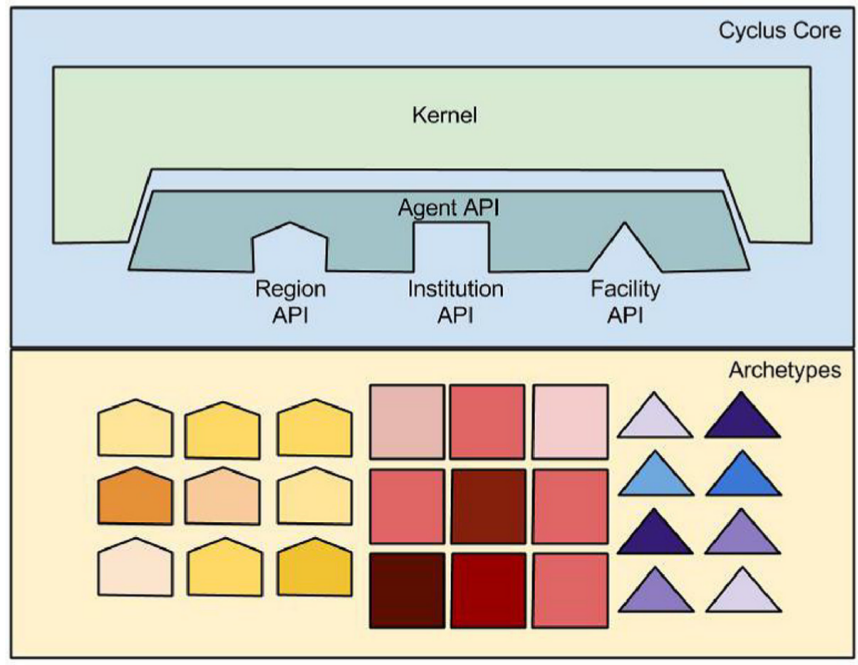
\includegraphics[width=\textwidth]{cyclus_core.png}
    \end{center}
    \caption{The \Cyclus core provides APIs that the archetypes
            can be loaded into the simulation modularly
            \cite{huff_fundamental_2016}.}
    \label{fig:core}
\end{figure}

Due to this modularity in the \Cyclus framework, the developed
model in this work is implemented independently without
having to modify the \Cyclus source code. The new facility archetype
is written in Python and implemented through the \Cyclus API.
